\section{Differenzialrechnung im Komplexen}
\subsection{Komplexe Zahlen}
\begin{satz}
	Es gibt einen komplexen Körper $\mathds{C}$ mit den folgenden Eigenschaften:
	\begin{itemize}
		\item[1)]
		$\mathds{R}$ ist ein Unterkörper von $\mathds{C}$, d.h. $\mathds{R} \subset \mathds{C}$ und Addition, Multiplikation auf $\mathds{R}$ enstehen durch Einschränkung der Addition, Multiplikation auf $\mathds{C}$
		\item[2)]
		Die Geichung $ x^2 + 1 = 0$ besitzt genau zwei Lösungen
		\item[3)]
		Sei i eine der beiden Lösungen. dann ist die Abbildung:
		\begin{eqnarray*}
			\mathds{R} \times \mathds{R} \to  \mathds{C} \\
			(x,y) \mapsto x+ iy
		\end{eqnarray*}
		
		bijektiv.\\
	\end{itemize}
\end{satz}

\begin{bew}
Wir versehen die Menge $\mathds{C} := \mathds{R} \times \mathds{R}$ mit der Addition $(x,y) + (u,v) := (x+u,y+v)$ und mit der \\
Multiplikation $(x,y)* (u,v) = (xu-yv, xv+yu) \qquad \forall (x,y),(u,v) \in \mathds{R} \times \mathds{R}$\\
\end{bew}
\textbf{zz:}
\begin{itemize}
	\item[1)] Assoziativität
	\item[2)] Kommutativität 
	\item[3)] Distributivität 
	\item[4)] neutrales Element\\
	0 := (0,0), 1:= (1,0)
	\item[5)] inverses Element\\
	-z=(-x,-y), ...
\end{itemize}


$\mathds{R}$ ist Unterkörper von $\mathds{C}$. Es gilt:\\
\begin{eqnarray*}
	(a,0)(x,y) &=& (ax,ay)\\
	\text{d.h. }(a,0)(b,0)&=&(ab,0)\\
	(a,0)+(b,0) &=& (a+b,0)
\end{eqnarray*}

$\Rightarrow \mathds{C}_{\mathds{R}}:= \{(a,0) \in \mathds{C}\}$ ist ein Unterkörper versehen mit Addition und Multiplikation durch Einschränkung, isomorph zu $\mathds{R}$.\\
Wir identifizieren (a,0) $\in \mathds{C}$ mit $a \in \mathds{R}$.\\

\begin{definition}
	$\mathds{C}$ heißt \textbf{Körper der komplexen Zahlen}.\\
	$i := (0,1)$ heißt \textbf{imaginäre Einheit}.
\end{definition}

In der Darstellung $z=x+iy \in \mathds{C}$, heißt x der \textbf{Realteil von z} und y der \textbf{Imaginärteil von z}.\\
Wir schreiben:
\begin{eqnarray*}
x= Re(z)\\
y = Im(z)
\end{eqnarray*}
Ist $Re(z) = 0$, dann heißt z \textbf{rein imaginär}.\\
Wir definieren: $\overline{z}= x-iy$ und nennen $\overline{z}$ die zu \textbf{z konjugiert komplexe Zahl}.\\
\begin{itemize}
	\item $\overline{\overline{z}} = z$
	\item $\overline{z \pm w} = \overline{z} \pm \overline{w}$
	\item $Re(z) = \frac{1}{2}(z + \overline{z}), \qquad Im(z)= \frac{1}{2}i(z-\overline{z})$
	\item $z=\overline{z} \Leftrightarrow z \in \mathds{R}\qquad z=-\overline{z} \Leftrightarrow z \in i\mathds{R}$
\end{itemize}

\begin{bemerkung}
\begin{eqnarray*}
	\text{für } z,w \in \mathds{C} \text{ und } n,m \in \mathds{N} \text{ gilt:}\\
	z^n &:=& \underbrace{z*z *\cdots z}_{n} \\
	z^0 &:=& 1\\
	z^{-n} &:=& (z^{-1})^{n}, n>0, z \neq 0\\
	\Rightarrow \qquad z^m z^n&=&z^{n+m}\\
	(z^m)^n &=& z^{nm}\\
	z^n w^n &=& (zw)^n\\
	(z+w)^n &=& \sum^n_{k=0} z^k w^{n-k}\\
\end{eqnarray*}

...\\
\end{bemerkung}

Die komplexe Konjugation ist also ein involutorischer Körperautomorphismus mit Fixkörper $\mathds{R}$.\\
\begin{definition}
	Da $z\overline{z} = x^2+y^2$ reell und nicht negativ ist, definieren wir den Betrag von z durch: $|z|:= \sqrt{z\overline{z}}$
\end{definition}

\textbf{Lemma: }\\
Es gilt:
\begin{itemize}
	\item
	$|z| \geq 0, |z| = 0 \Leftrightarrow z = 0$
	\item
	$|zw| = |z||w|$
	\item
	$|Re(z) \leq |z|, |Im(z)| \leq |z|$
	\item
	 $|w+z| \leq |w|+|z|$
	 \item
	 $||z|-|w|| \leq |z-w|$
	 \item
	 $z^{-1} = \frac{\overline{z}}{|z|^2}$
\end{itemize}
\textbf{Beweis: }\\
1) bis 3) klar, 4), 5): Übungsaufgabe 6.\\
6) $z^{-1} =  \frac{x}{x^2 +y^2}- \frac{iy}{x^2+y^2} = \frac{\overline{z}}{|z|^2}$\\

\textbf{Bemerkung:}\\
Geometrische Veranschaulichung: \\
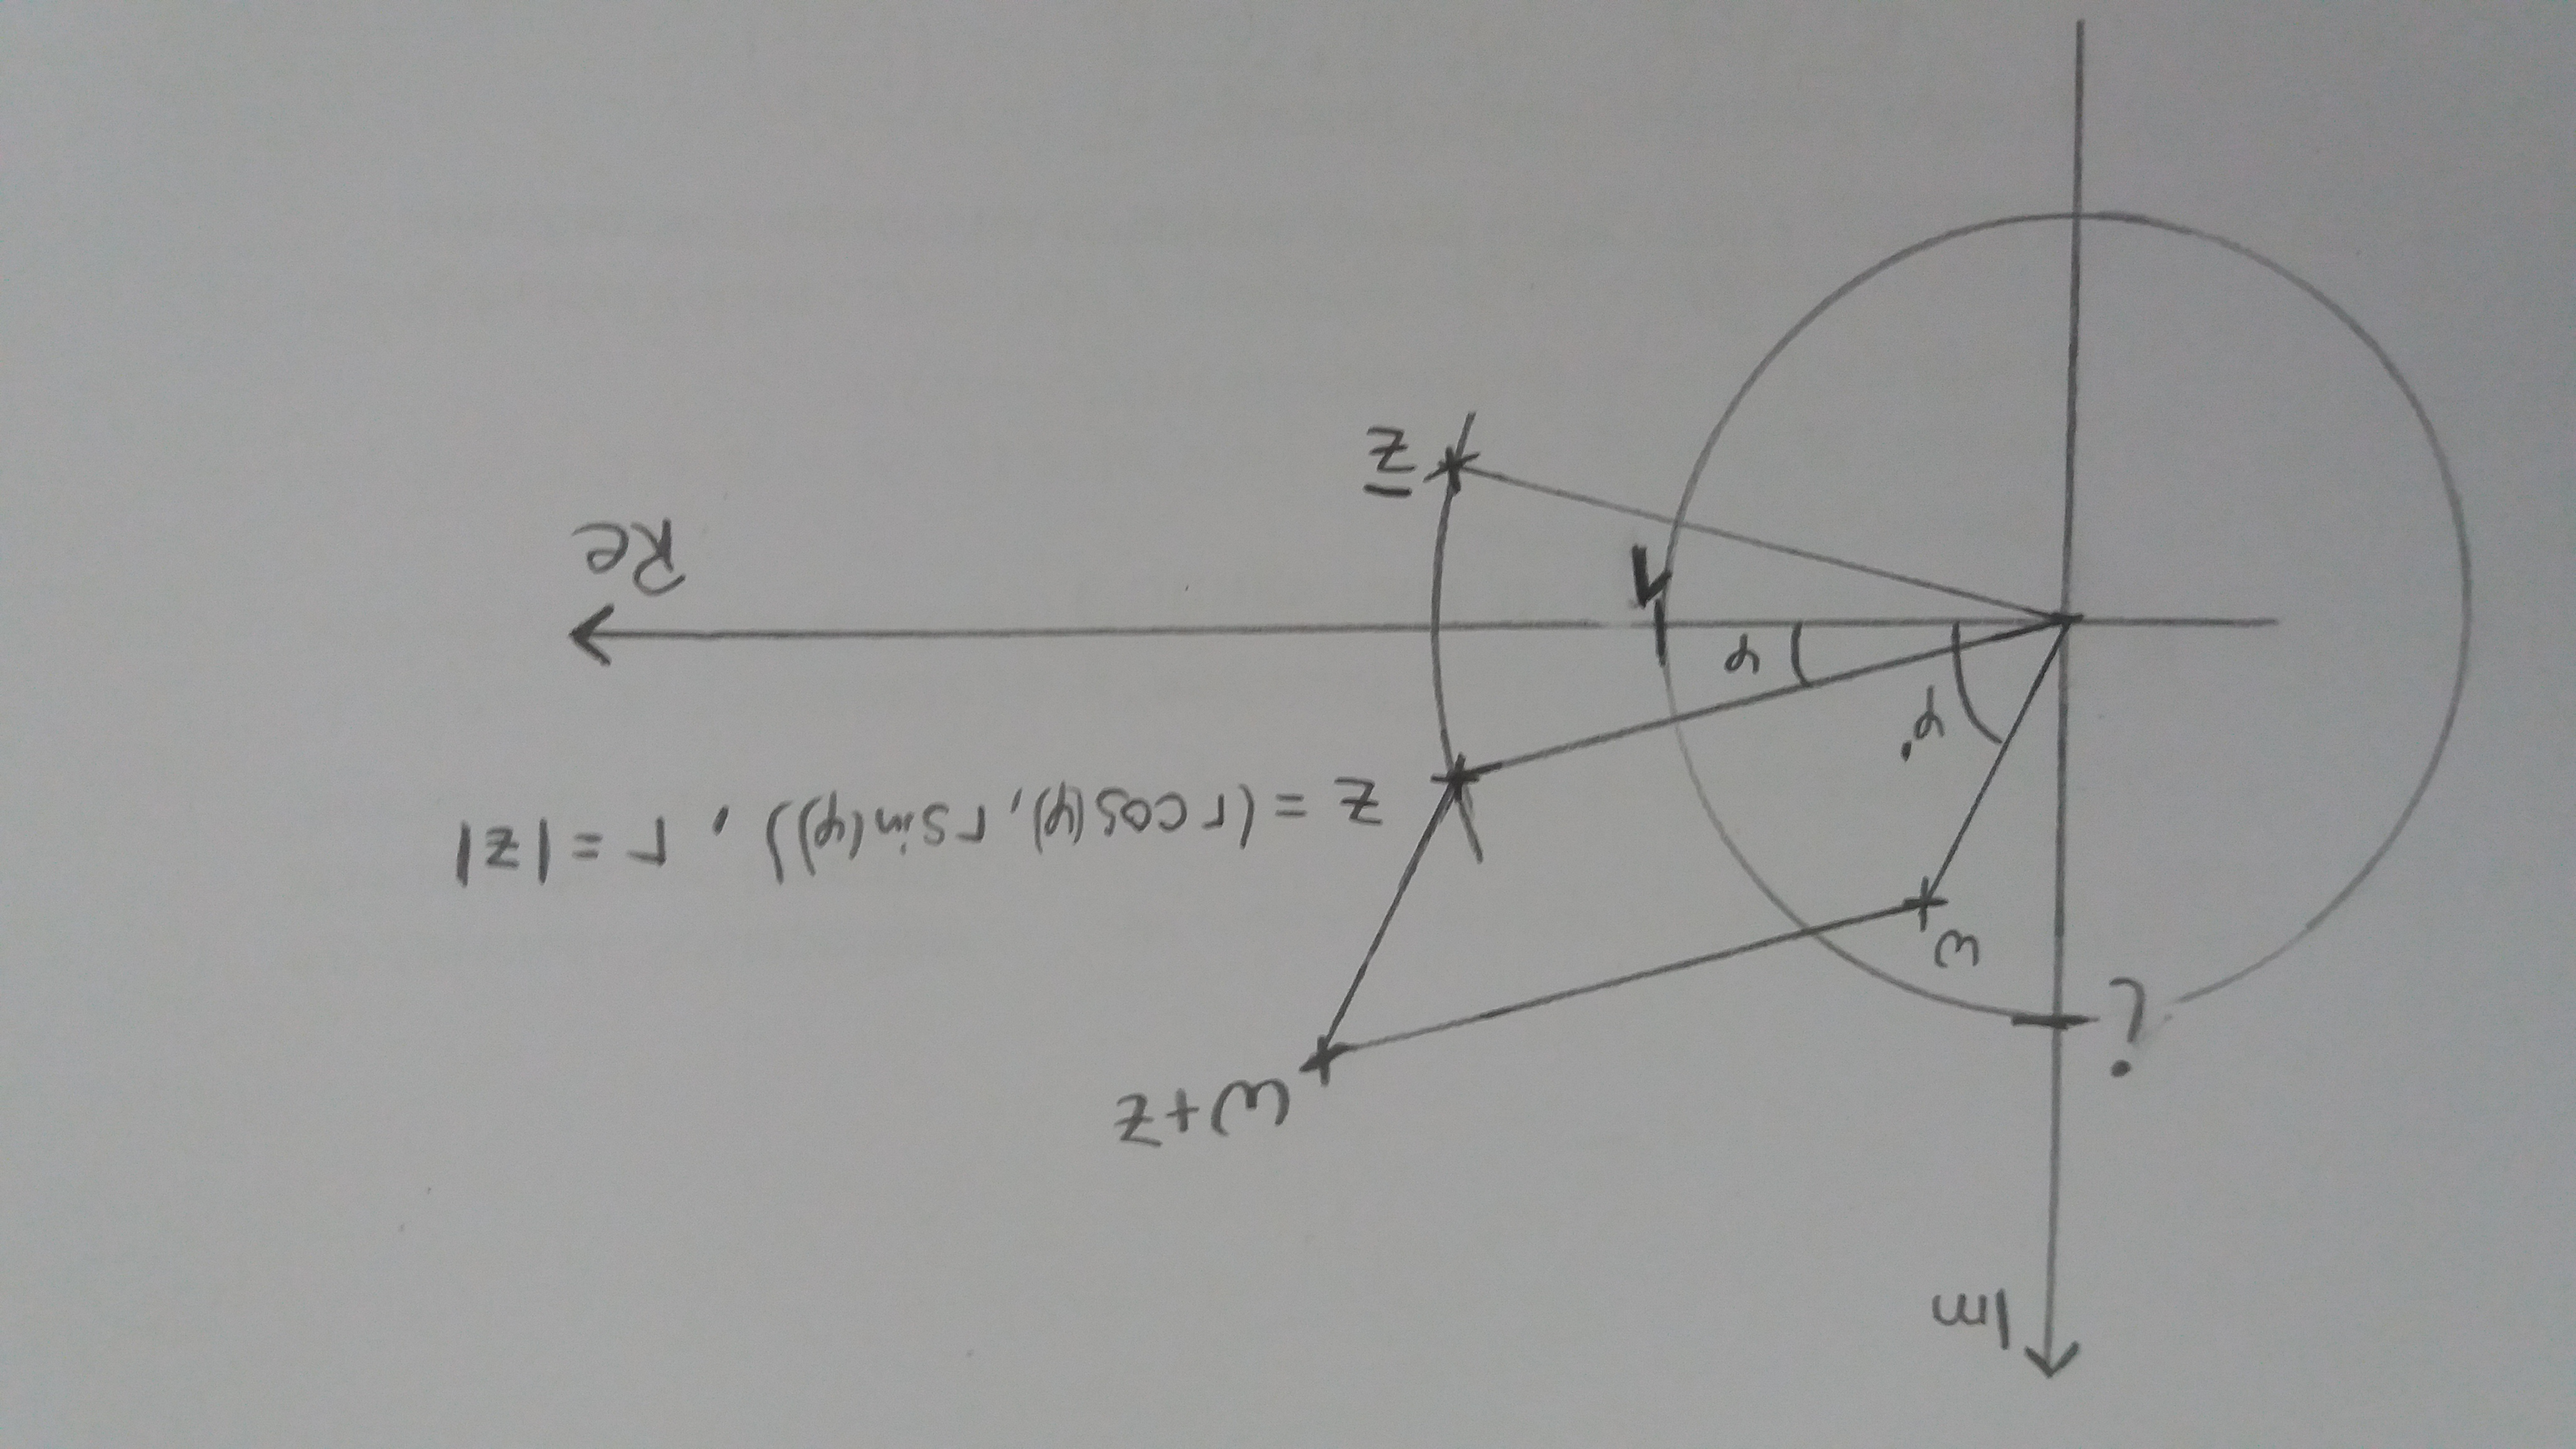
\includegraphics[scale=0.1, angle=180]{pics/Polar.jpg} \\

\textbf{Proposition: }\\
\begin{eqnarray*}
\mathds{R}^x_+ &=& \{z \in \mathds{C}| x > 0\} \\
\mathds{C}^x &=& \{ z \in \mathds{C} | z \neq 0\} =  \mathds{C} \setminus\{0\} 
\end{eqnarray*}

\begin{itemize}
	\item
	Die Polarkoordinatendarstellungsabbildung:
	\begin{eqnarray*}
	\mathds{R}^x_+ \times \mathds{C} \\
	(r,\varphi) \mapsto z = r(cos(\varphi),i sin(\varphi))
	\end{eqnarray*}
	ist surjektiv.
	\item
	Aus $z = z', d.h.\quad r(cos(\varphi, i sin(vaphi)) = r'(cos(\varphi', i sin(\varphi'))$\\
	...\\$r(cos(\varphi, i sin(\varphi))$
\end{itemize}
\textbf{Beweis:}
Aus reellen Analysis folgt: \\
jedes $z = (x,y) \neq (0,0)$ kann eindeutig geschrieben werden als $z = (r cos(\varphi), rsin(\varphi))$. \\
Daher ist r eindeutig bestimmt durch $r = \sqrt{x^2 + y^2}$ \\
$\varphi$ ist jedoch nur eindeutig bis auf ganzzahlig Vielfache von $2\pi$

\begin{definition}
	Sei $z \in \mathds{C}$. Jedes $\varphi \in  \mathds{R}$ mit $z =r(cos(\varphi, i sin(\varphi))  $ heißt ein \textbf{Argument von z}. Wir schreiben $\varphi = arg(z)$.
	Falls $\varphi \in (\-\pi,\pi]$ , heißt $\varphi$ \textbf{Hauptwert des Arguments von z}. Wir schreiben $\varphi = Arg(z)$.
\end{definition}
